\documentclass{report}
\usepackage{subcaption} 
\usepackage{graphicx}

\begin{document}
\begin{figure}
  \begin{subfigure}[b]{0.5\textwidth}
    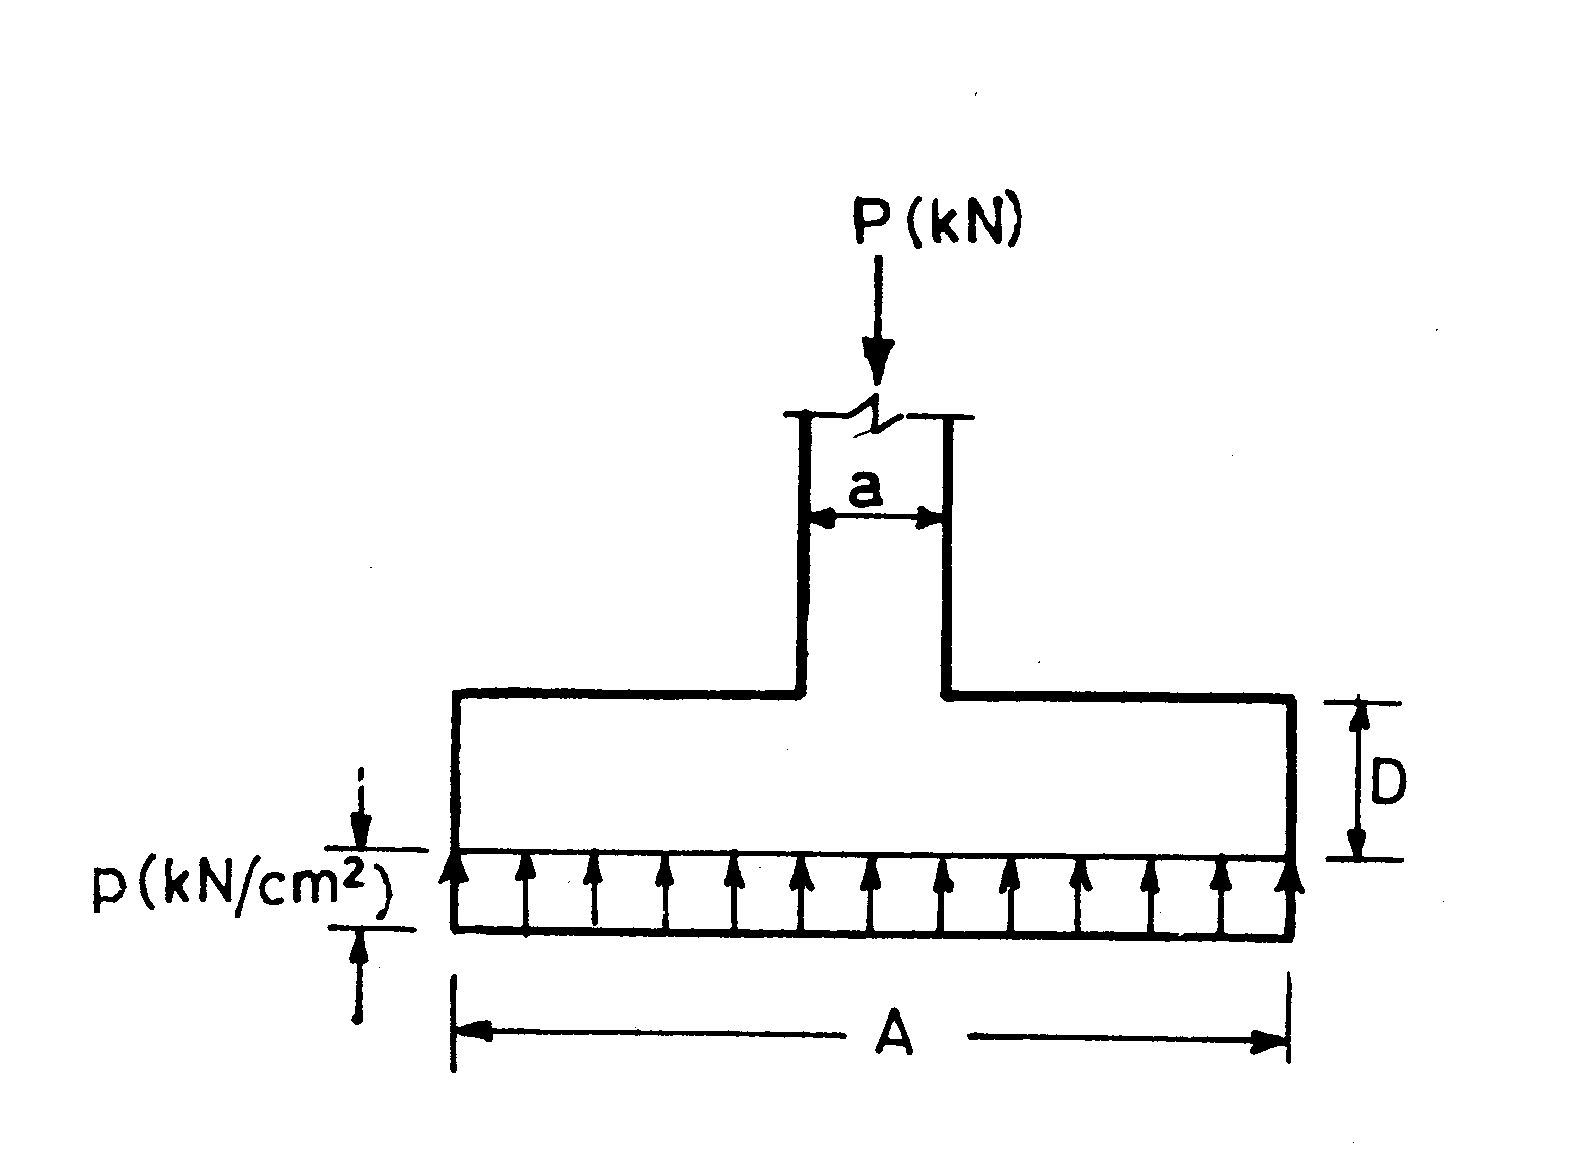
\includegraphics[width=\textwidth]{images/fig2291.png}
    \caption{Uniform deep footing}
    \label{fig:1}
  \end{subfigure}
  %
  \begin{subfigure}[b]{0.5\textwidth}
    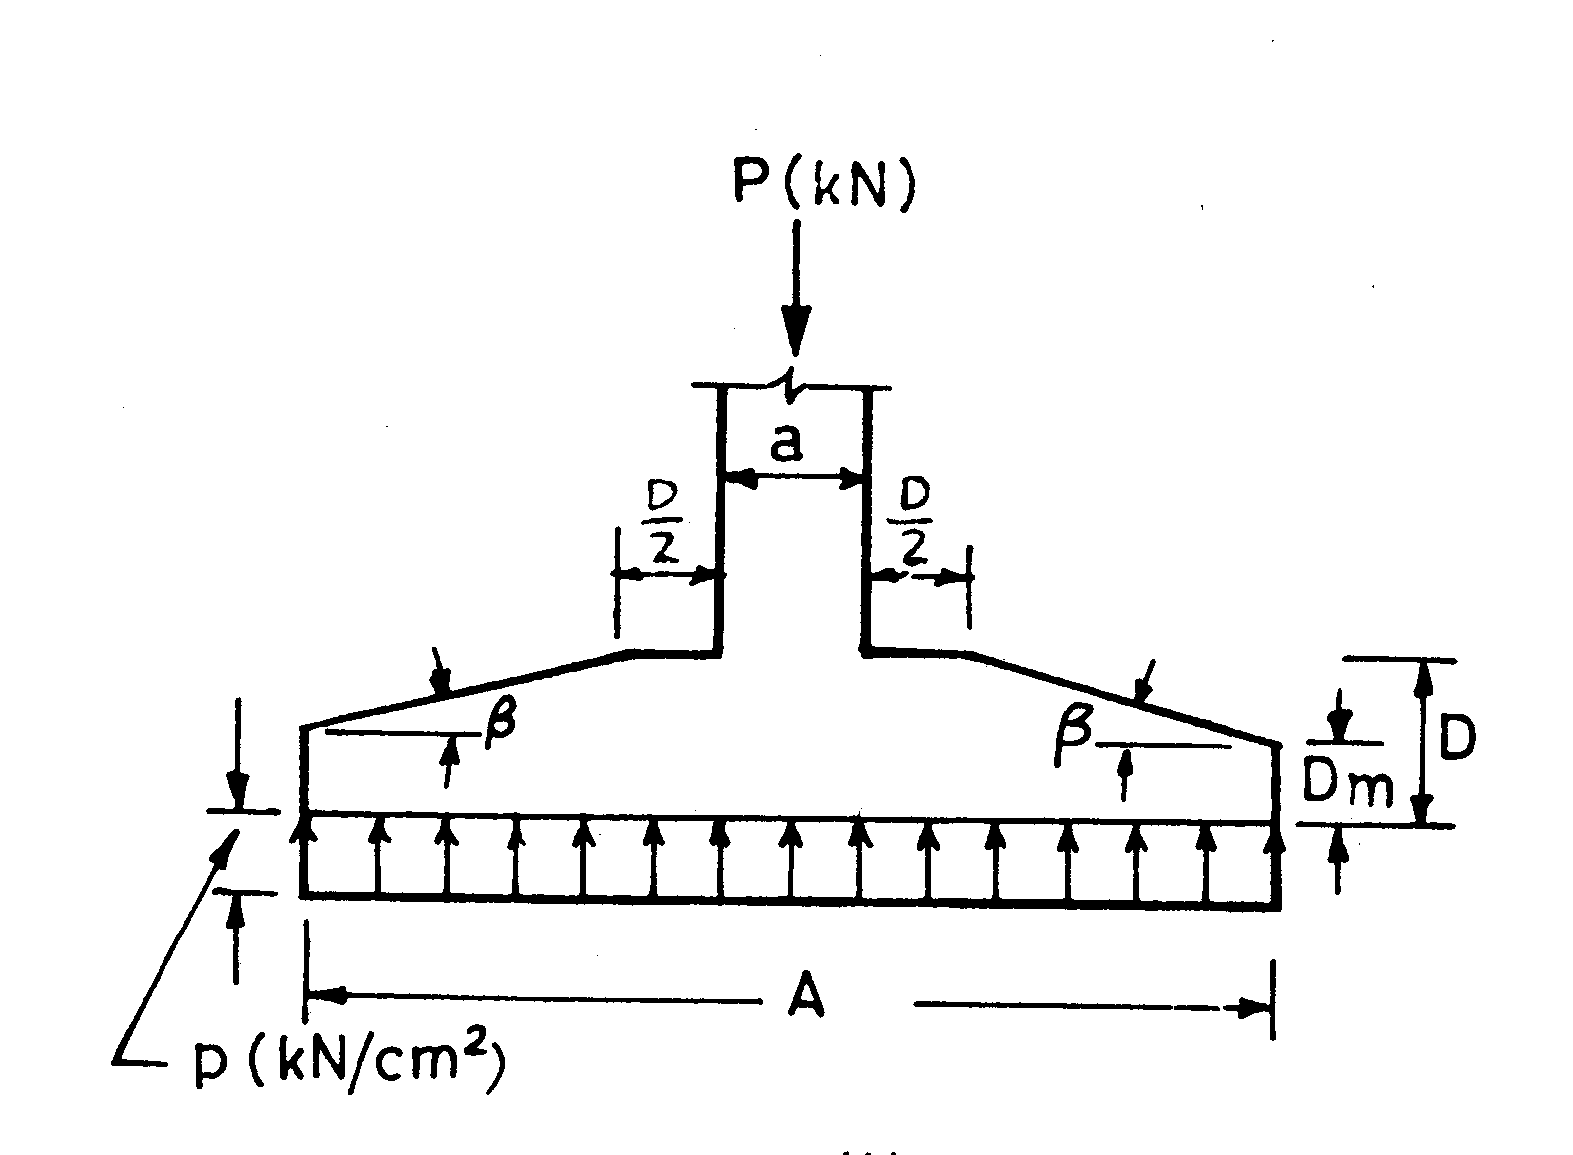
\includegraphics[width=\textwidth]{images/fig2292.png}
    \caption{Sloped footing( slope starting from D/2 away from the edge of column)}
    \label{fig:2}
  \end{subfigure}
 %
 \begin{subfigure}[b]{0.5\textwidth}
    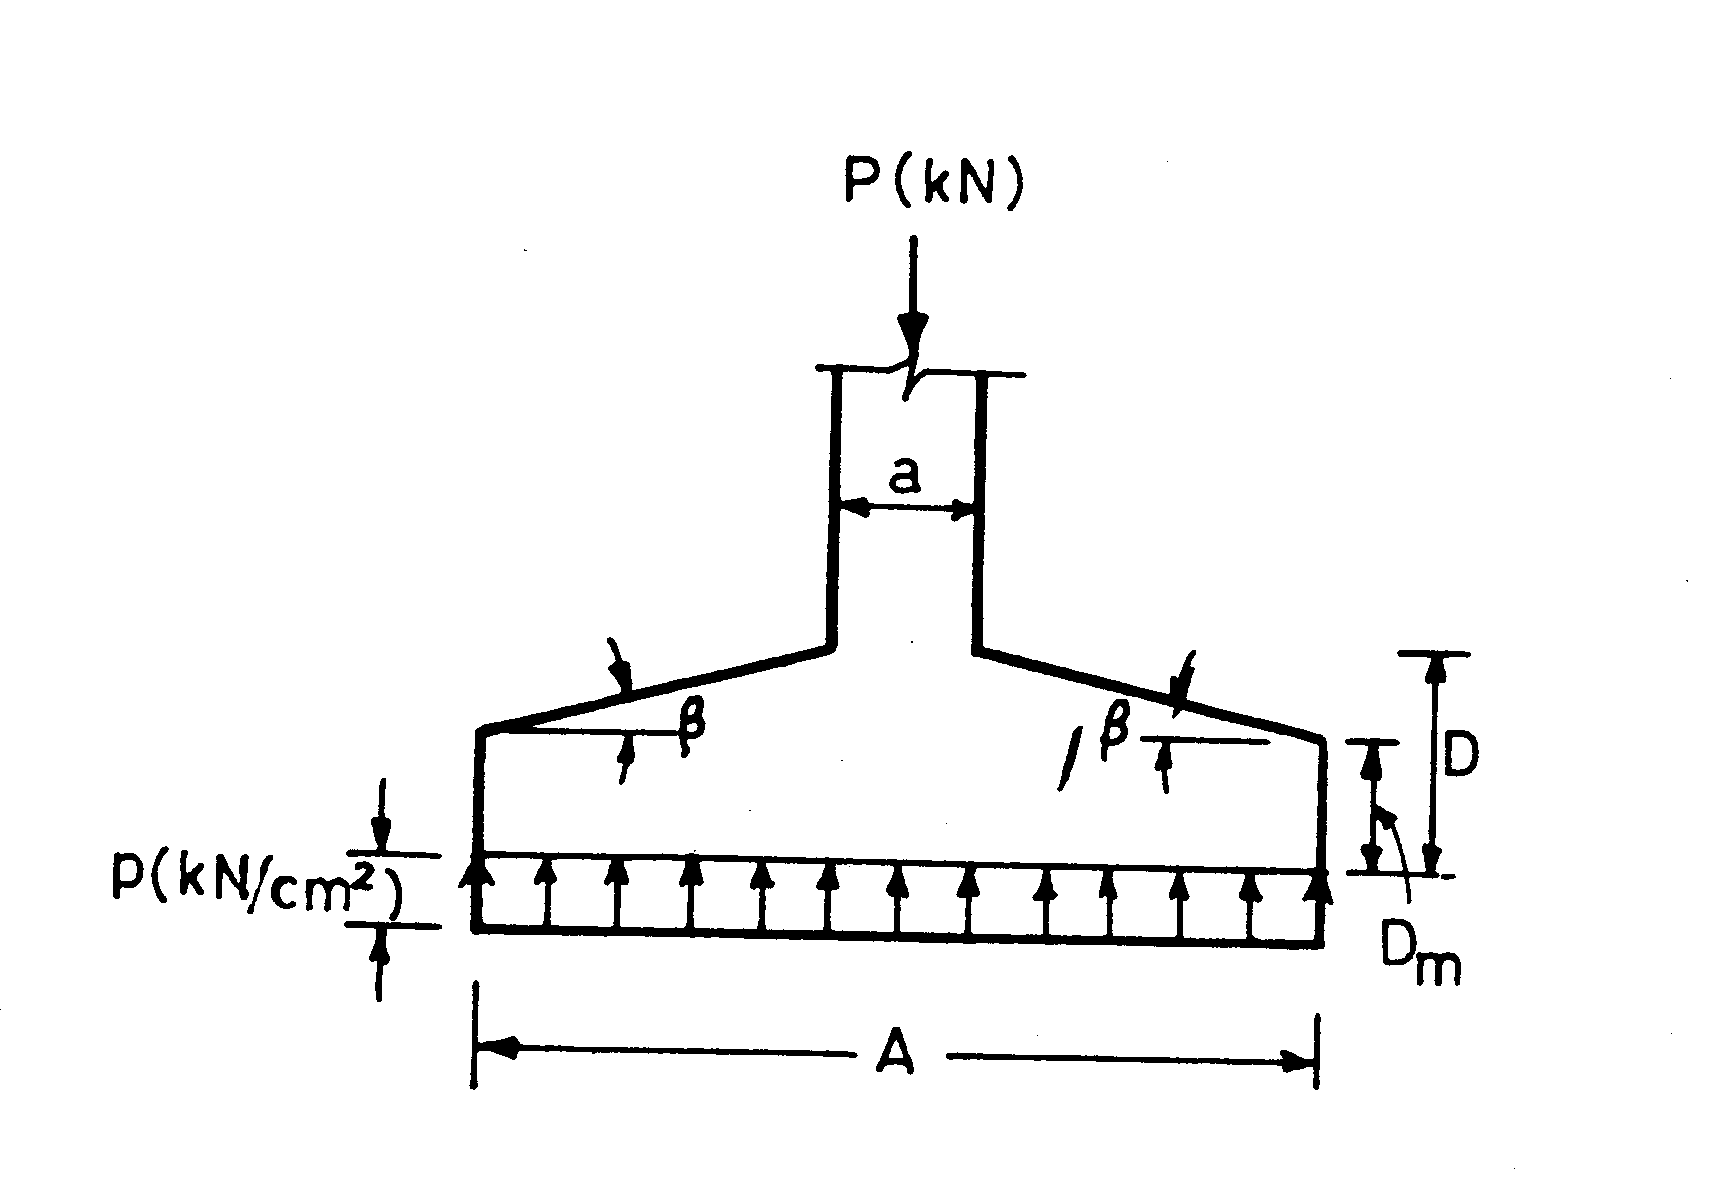
\includegraphics[width=\textwidth]{images/fig2293.png}
    \caption{Sloped footing (slope starting from the edge of column)}
    \label{fig:2}
  \end{subfigure}
 %
\begin{subfigure}[b]{0.5\textwidth}
    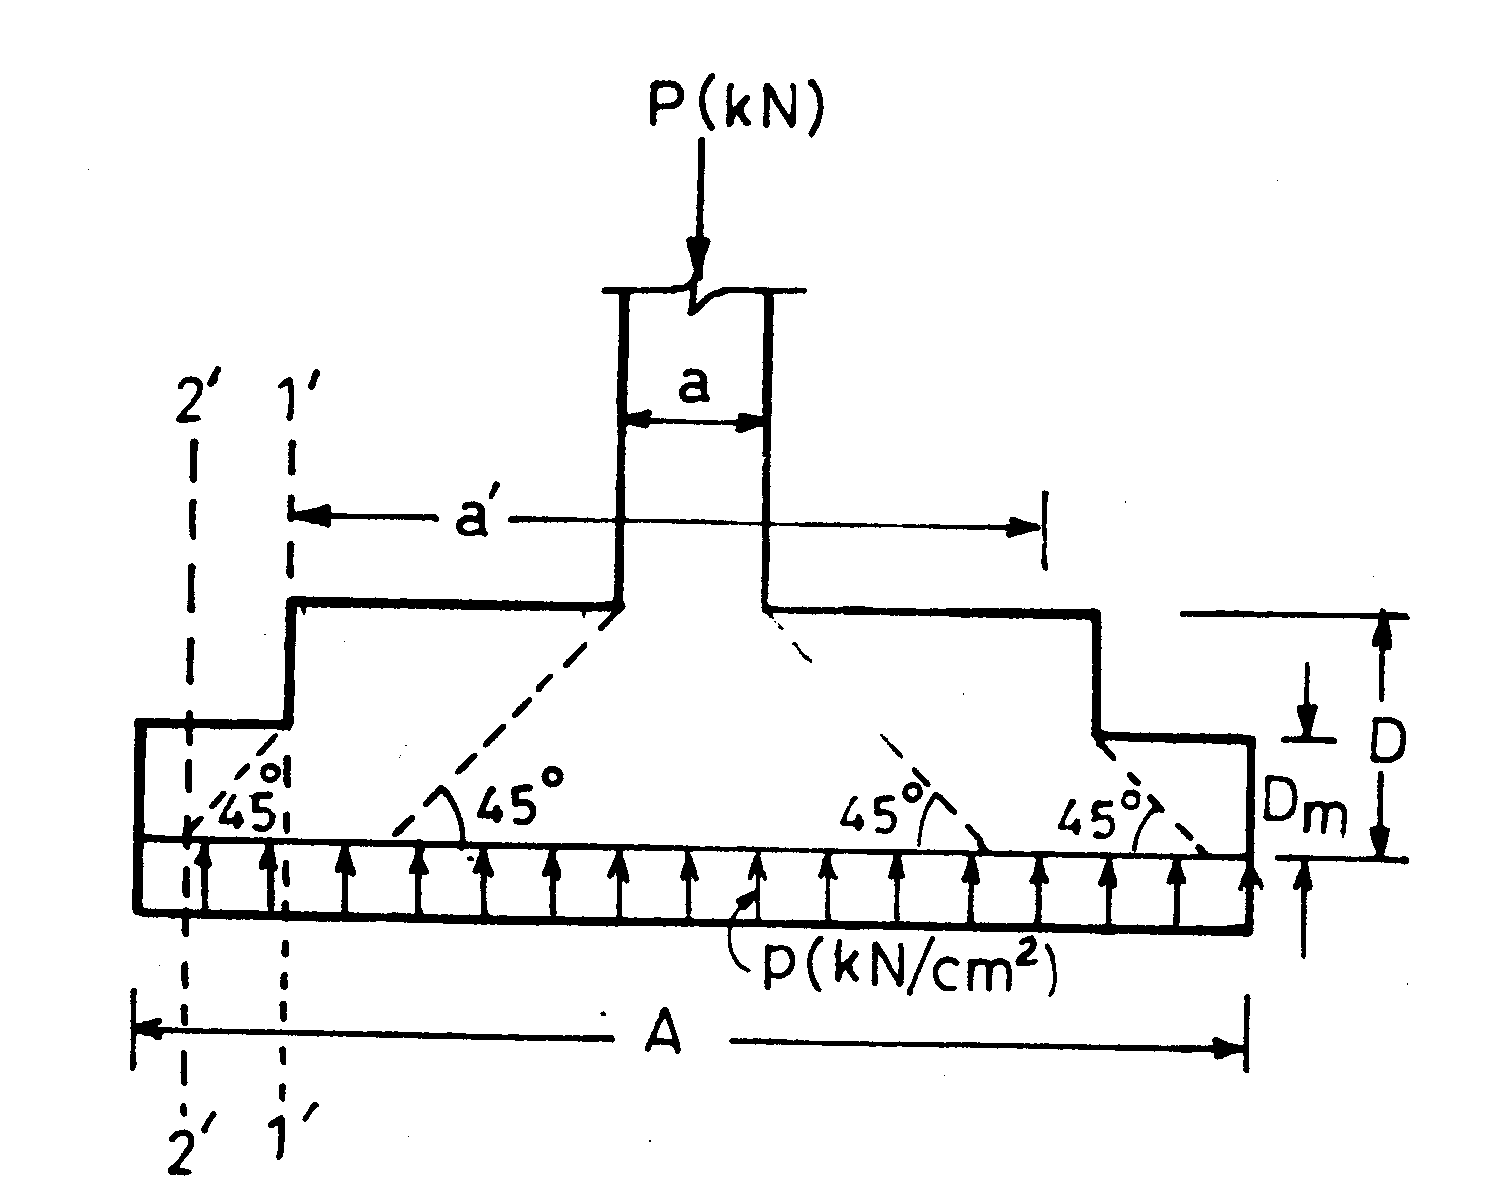
\includegraphics[width=\textwidth]{images/fig2294.png}
    \caption{Stepped footing}
    \label{fig:2}
  \end{subfigure}
\caption{Types of individual spread footing}
\end{figure}

THis is second figure which is inserted below the text.

\begin{figure}
  \begin{subfigure}[b]{0.5\textwidth}
    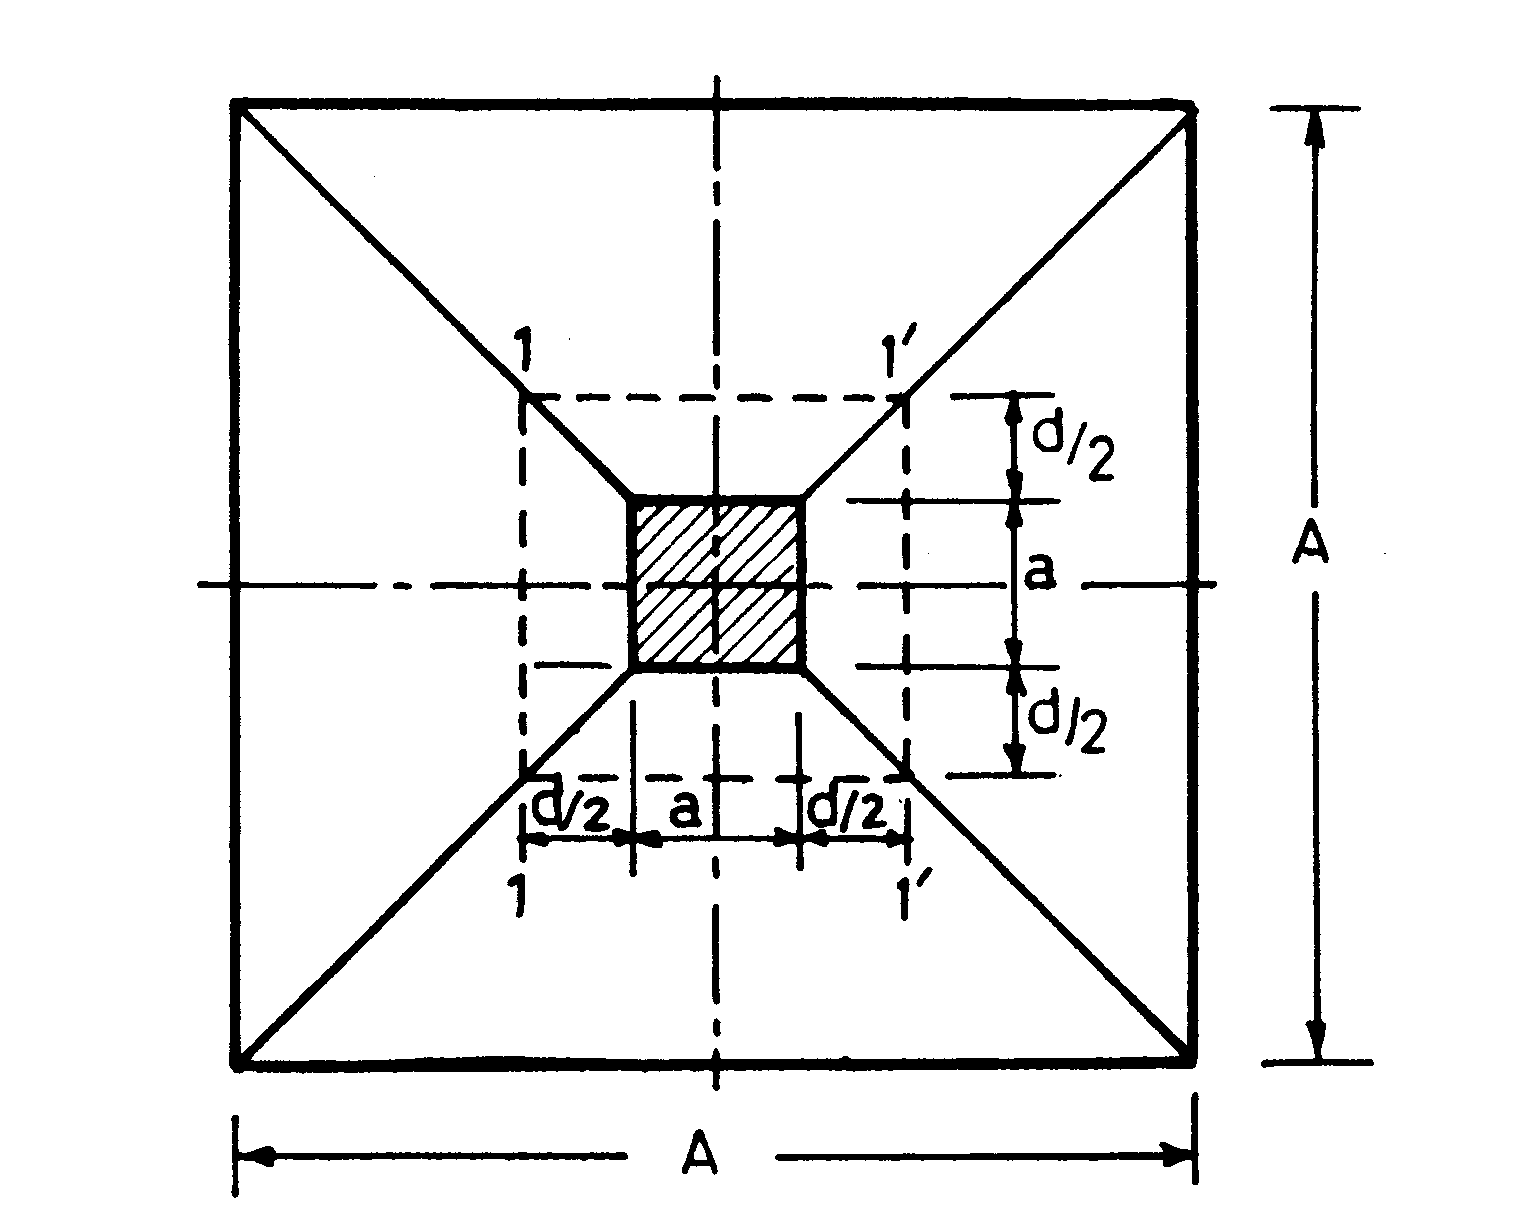
\includegraphics[width=\textwidth]{images/fig2301.png}
    \caption{Critical perimeter 1-1-1-1 in plan for perimeter shear}
    \label{fig:1}
  \end{subfigure}\\
  %
  \begin{subfigure}[b]{0.5\textwidth}
    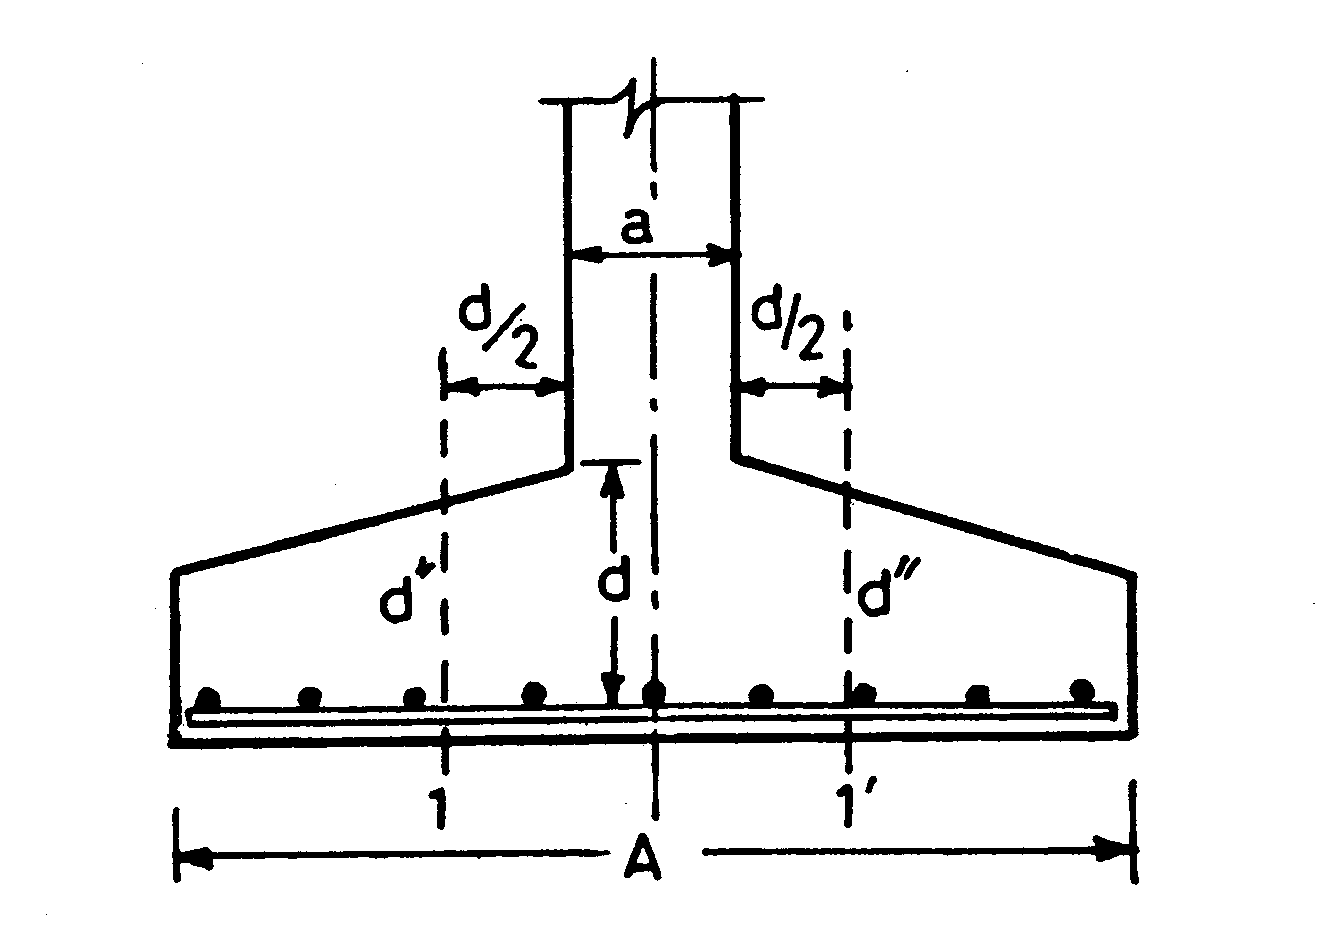
\includegraphics[width=\textwidth]{images/fig2302.png}
    \caption{Section of sloped footing showong reduced depth of perimeter shear}
    \label{fig:2}
  \end{subfigure}
\caption{Perimeter shear for square footing}
\end{figure}

this is thrid test
\begin{figure}[h]
  \centering
  \begin{subfigure}[b]{0.5\textwidth}
    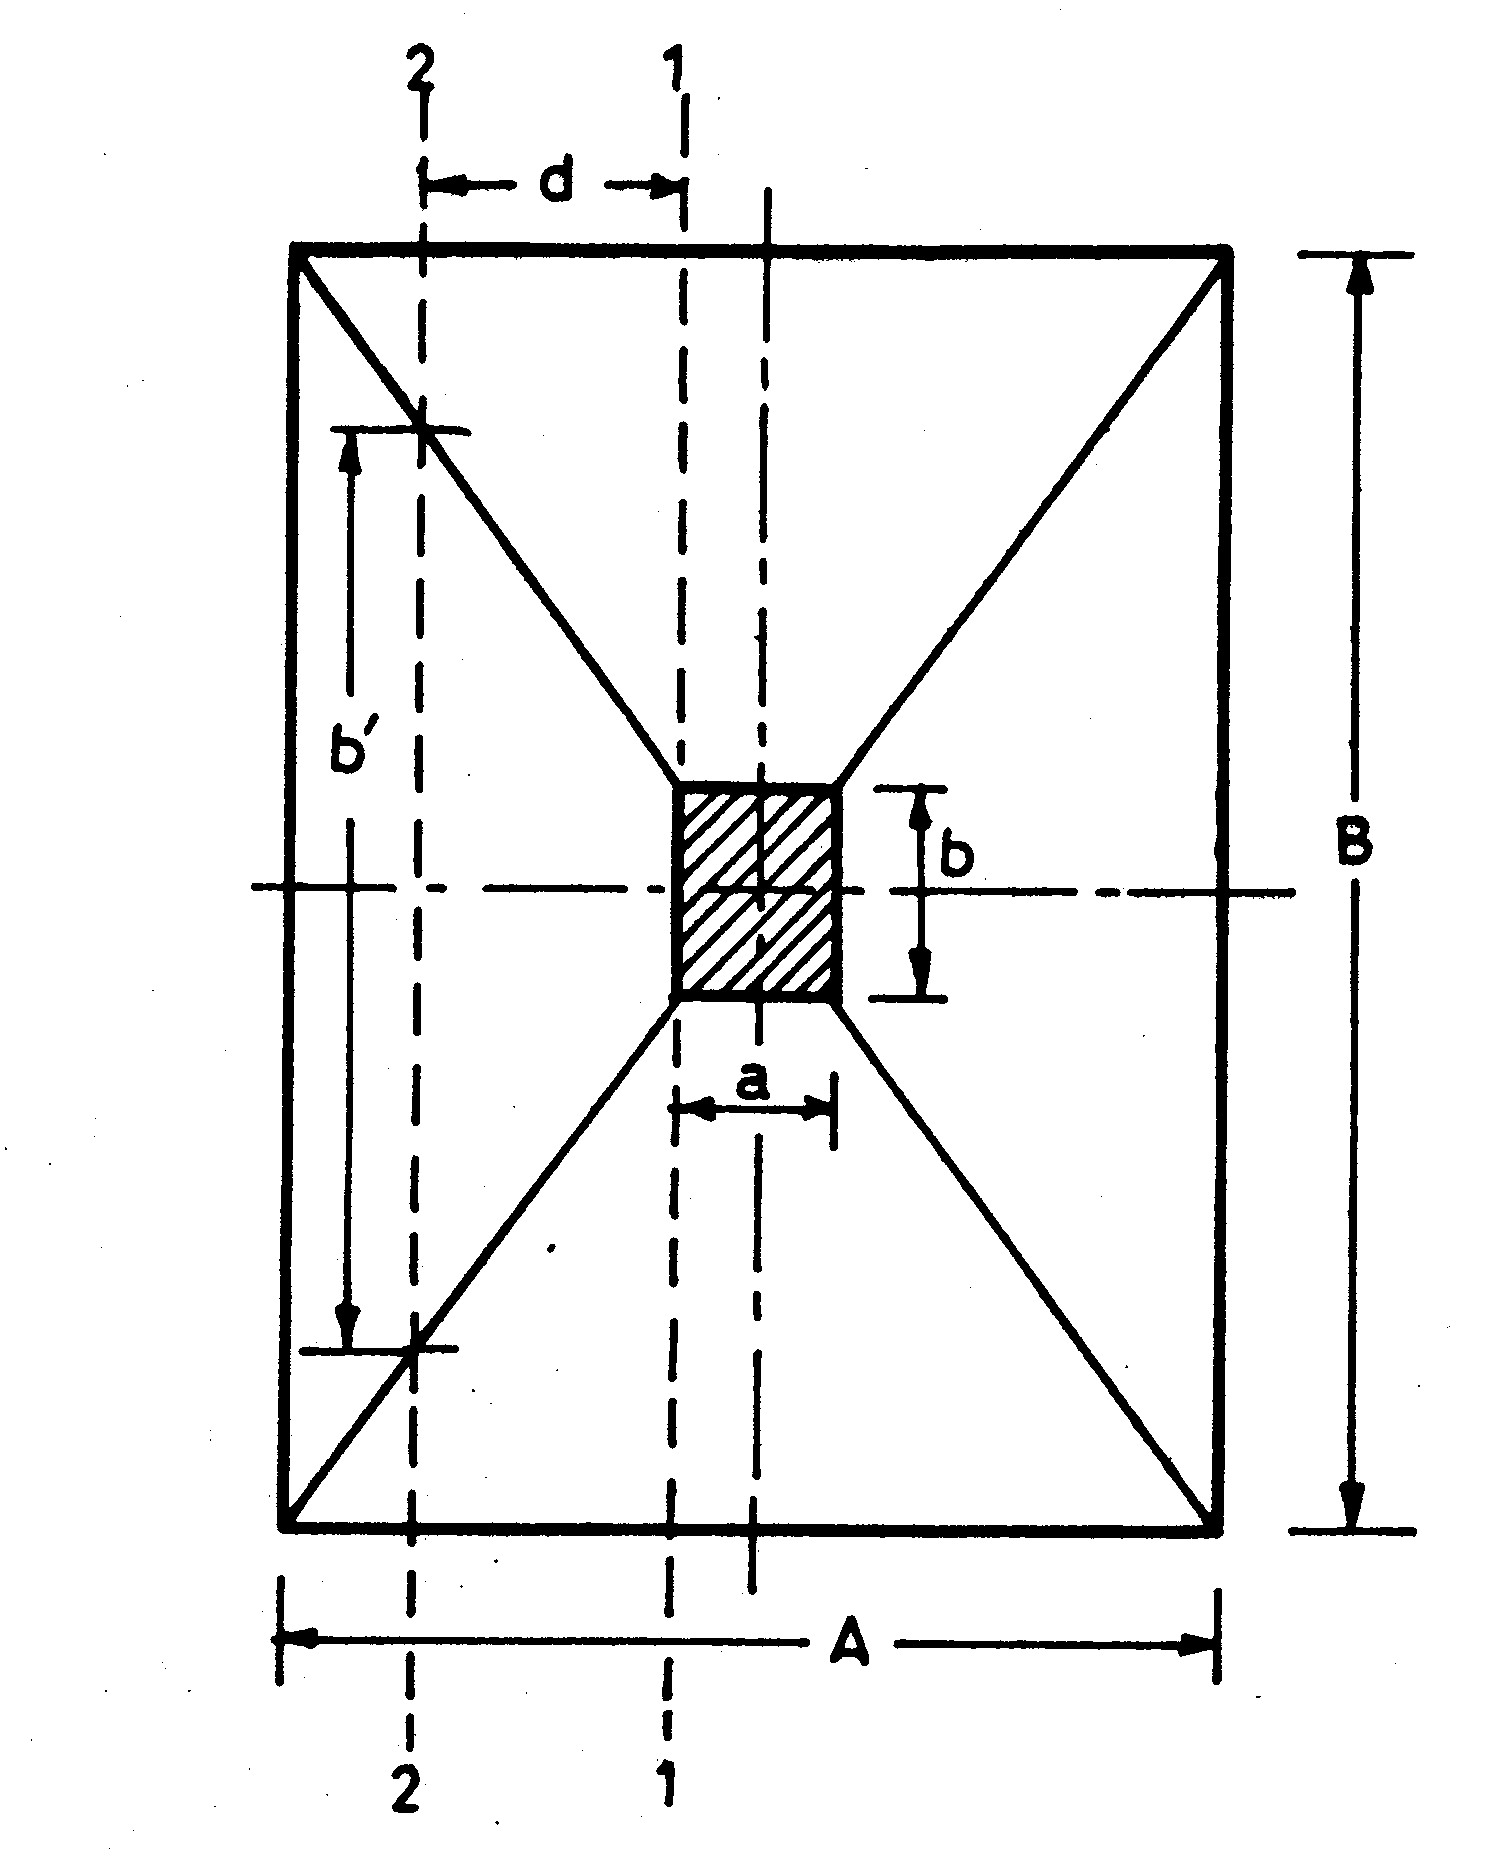
\includegraphics[width=\textwidth]{images/fig2321.png}
    \caption{Plan of sloped footing}
    \label{fig:1}
  \end{subfigure}\\
  %
  \begin{subfigure}[b]{0.5\textwidth}
    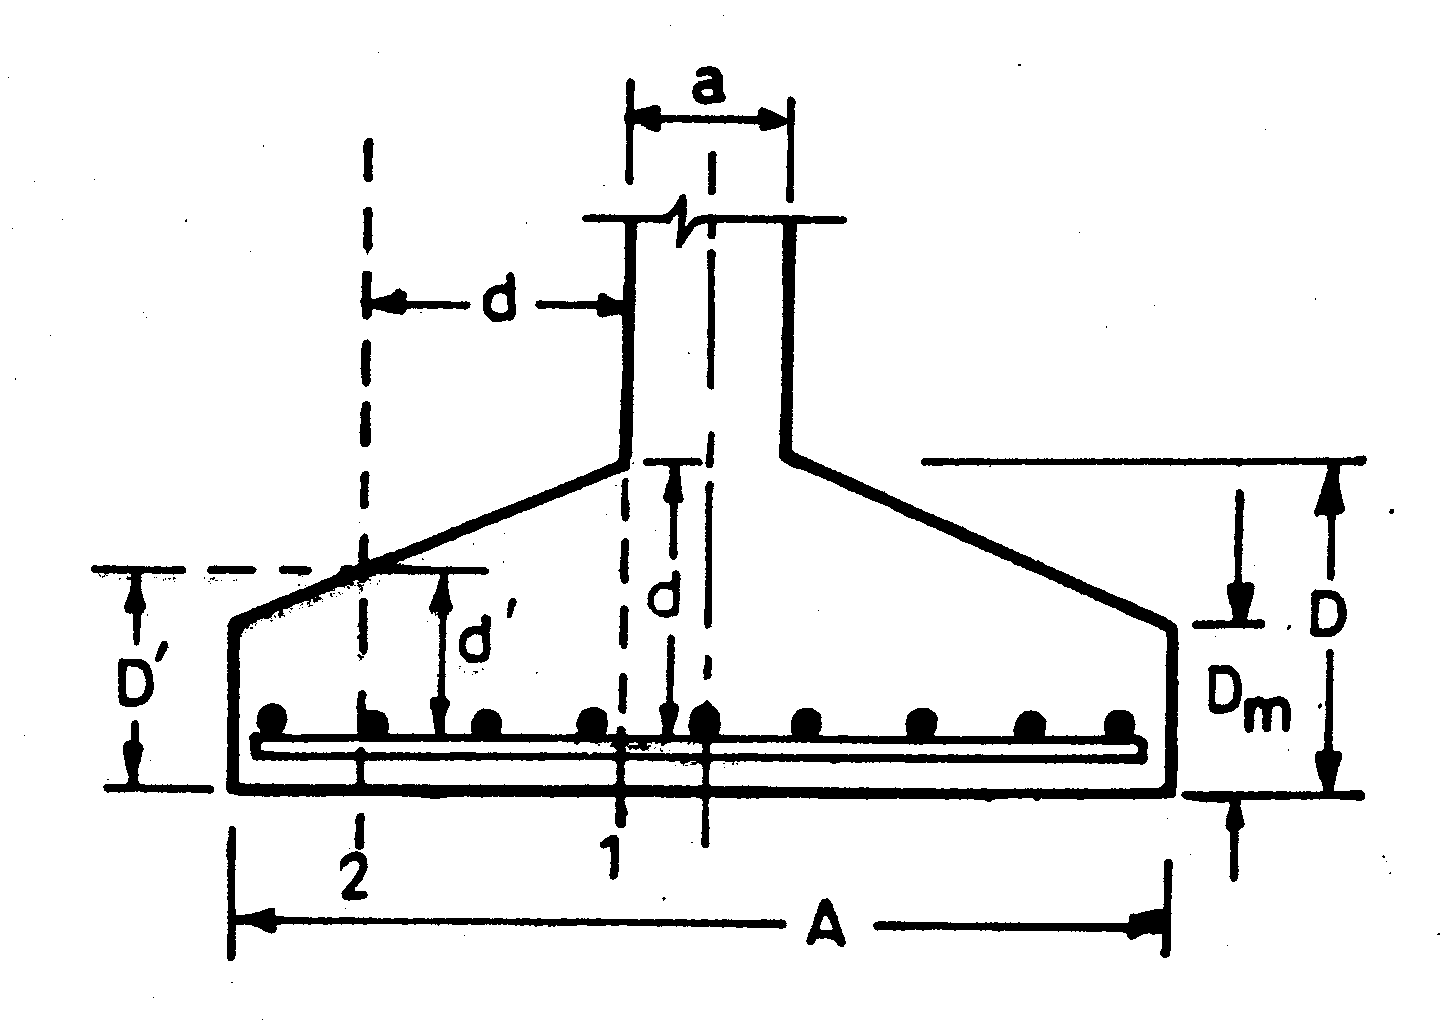
\includegraphics[width=\textwidth]{images/fig2322.png}
    \caption{Section of sloped footing}
    \label{fig:2}
  \end{subfigure}
\caption{Perimeter shear for square footing}
\end{figure}
\end{document}
